\documentclass[a4paper, 12pt]{article}
\usepackage[a4paper,left=2.5cm,right=3cm,top=2cm,bottom=2cm]{geometry}
\usepackage[ngerman]{babel}
\usepackage[utf8]{inputenc}
\usepackage[]{csquotes}
\usepackage[style=authoryear-comp,backend=biber]{biblatex}
\usepackage{mathptmx}
\usepackage[T1]{fontenc}
\usepackage{relsize}
\usepackage{graphicx}
\usepackage[]{blindtext}
\graphicspath{ {images/} }

\addbibresource{sources.bib}

\author{Lars Eppinger}
\title{Quantifizierung von Code-Qualität mithilfe statischer Code-Analyse}
\date{1. Juni 2020}

\begin{document}
\begin{titlepage}
    \begin{center}
        \vspace*{1cm}
        
        \Huge
        \textbf{Quantifizierung von Code-Qualität mithilfe statischer Code-Analyse}
        
        \vspace{0.5cm}
        \LARGE
        Sind Tools zur statischen Code-Analyse ein akkurater Weg zur Quantifizierung von Code-Qualität in der objektorientierten Programmierung?
        
        \vspace{1.5cm}
        
        \textbf{Lars Eppinger}

        \Large
        178121\\
        DAI-17
        
        \vfill
        
        Fachbeitrag zur Modulprüfung\\Wissenschaftlich angeleitete Berufspraxis
        
        \vspace{0.8cm}
        
        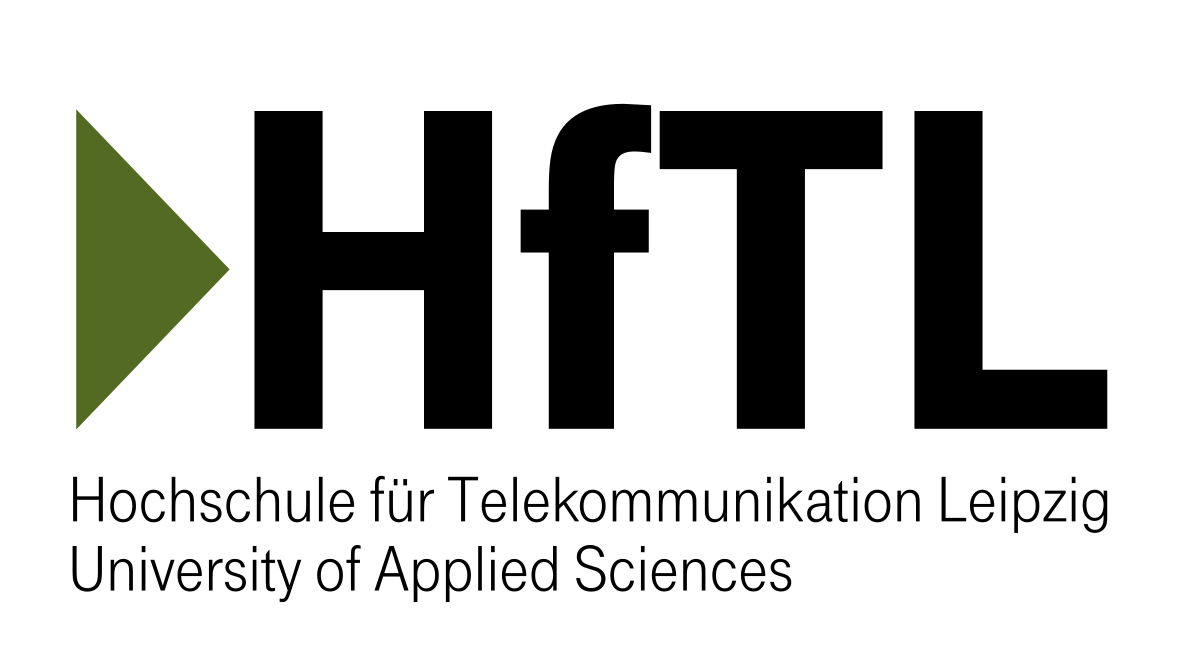
\includegraphics[width=0.4\textwidth{}]{university.png}
        
        \Large
        Hochschule für Telekommunikation Leipzig\\
        1. Juni 2020
        
    \end{center}
\end{titlepage}
\tableofcontents
\newpage

\section{Einführung}
Code-Qualität ist einer der entscheidenden Faktoren über Sicherheit, Wartbarkeit und Maintainability von Softwareprojekten. 
Durch neue Ansätze in der Softwareentwicklung, speziell der agilen Softwareentwicklung, ist es immer wichtiger, hohe Qualität in einer Codebasis sicherzustellen, um die Umsetzung neuer Anforderungen so schnell und fehlerfrei wie möglich zu gestalten.
Immer häufiger kommen für diesen Zweck Tools zur statischen Code-Analyse zum Einsatz.
In dieser Arbeit wird die Frage geklärt, ob diese Tools geeignet sind, um die Qualität einer Codebasis in der objektorientierten Progammierung zu quantifizieren.

\section{Code-Qualität}
\subsection{Definition}
Als Definitionskriterien für Code-Qualität verwendet diese Arbeit die Attribute für Code-Qualität von \textcite{Linda_softwarequality} und den daraus abgeleiteten Metriken.
Diese basieren auf den Metriken für das Design von objektorientierter Software, welche von \textcite{Metrics_OO_design} erörtert wurden.
Metriken für die Quantifizierung von Code-Qualität müssen nach \textcite{Linda_softwarequality} dazu geeignet sein, die folgenden Attribute eines System zu evaluieren:
\begin{itemize}
    \item Effizienz -- Sind die Konstrukte effizient entworfen?
    \item Komplexität -- Könnten die Konstrukte effektiver genutzt werden, um architekturelle Komplexität zu reduzieren?
    \item Verständlichkeit -- Erhöht das Softwaredesign die psychologische Komplexität?
    \item Wiederverwendbarkeit -- Lässt das Softwaredesign zu, dass Komponenten wiederverwertet werden können?
    \item Testbarkeit -- Lässt die Struktur einfaches Testing zu?
\end{itemize}
\subsection{Metriken}
Um diese Attribute zu evaluieren, eigenen sich die folgenden Metriken:

\paragraph{Zyklomatische Komplexität (McCabe-Metrik)}
Mit der von von Thomas J. McCabe begründeten zyklomatischen Komplexität lässt sich die Komplexität von Methoden beschreiben. 
Zyklomatische Komplexität bezieht sich hierbei auf Kontroll-Statements in Methoden, beispielsweise \enquote{if-else} oder \enquote{switch-case}-Statements.
Die zyklomatische Komplexität ist hierbei definiert als die Anzahl linear unabhängiger Pfade im Kontrollflussgraphen der zu bewertenden Methode. 
Sie lässt sich wie folgt berechnen: $M = b + p$, wobei $b$ die Anzahl der Binärverzweigungen und $p$ die Anzahl der Kontrollflussgraphen darstellt.
Bei der Betrachtung einer einzelnen Methode ist das $p$ stets 1, da ein Kontrollflussgraph eine Methode beschreibt.
Eine Binärverzweigung ist eine Verzweigung des Kontrollflusses mit lediglich zwei Entscheidungsmöglichkeiten, etwa ein \enquote{if}-Statement.
Verzweigungen mit mehreren Entscheidungsmöglichkeiten, etwa ein \enquote{switch-case}-Statement, lassen sich mittels der Formel $b = z - 1$ zu Binärverzweigungen umrechnen,  wobei $z$ die Anzahl der Zweige darstellt \parencite{McCabe_complexity}.

\paragraph{Größe}
Die Größe einer Methode spielt zum Verständnis dieser eine entscheidende Rolle. Kürzere Funktionen sind einfacher zu verstehen. 
Hierbei fallen Lines of Code (LOC), Leerzeilen und die Anzahl an Anweisungen ins Gewicht. 
Je nach verwendeter Programmiersprache können hier startke Variationen bezüglich dessen auftreten, was \enquote{verständlicher} Code ist (\textcite{Kim_software_implementation}, \textcite{Lorenz_object_oriented_software_metrics}, \textcite{Linda_softwarequality}).

\paragraph{Anteil an Kommentaren}
Kommentare können Entwicklern dabei helfen, geschriebenen Code zu verstehen, da sie komplexe Vorgänge näher erläutern können. 
\textcite{Linda_softwarequality} referenzieren hier einen Anteil von 30\%, welcher aus Kommentaren bestehen sollte.
Allerdings lässt sich Code-Qualität in der Realität nur schwer anhand von Anzahl an Kommentaren quantifizieren, da die reine Quantität an Kommentaren nichts über deren Qualität aussagen kann.
Kommentare können problematisch werden, da sie falsch, veraltet oder irreführend sein können \parencites[85]{Martin2009}.
Robert C. Martin beschreibt Kommentare als einen Weg, \enquote{unsere Unfähigkeit aus[zu]gleichen, uns in unserem Code klar auszudrücken} \parencites[85]{Martin2009}.
Mit dieser Aussage bezieht sich Martin darauf, dass Kommentare primär ein Hilfsmittel sind, um unverständlichen Code zu verstehen.
Das übergeordnete Ziel ist demnach, Code zu schreiben, welche bestenfalls ohne Kommentare zu verstehen ist.
Aus diesem Grund muss eine niedrige Anzahl an Kommentaren nicht zwangsläufig auf schlecht dokumentierten Code hinweisen, sonder kann auch ein Indikator dafür sein, dass die zu bewertende Codebasis so verständlich ist, dass eine weitere Erläuterung durch Kommentare nicht vonnöten ist.
Daher wird diese Metrik in dieser Arbeit nicht als Indikator für Code-Qualität herangezogen.


\section{Statische Code-Analyse}
\subsection{Stand der Technik}
\blindtext

\section{Problematik}
\blindtext

\newpage
\printbibliography
\end{document}